% select document class
\documentclass[11pt,a4paper]{article}

% include packages
\usepackage[T1]{fontenc}
\usepackage[ngerman]{babel}
%\usepackage[autostyle=true]{csquotes}
\usepackage{amsmath}
\usepackage{amssymb}
\usepackage{mathtools}
\usepackage{graphicx}
\usepackage{hyperref}
%\usepackage{siunitx}
\usepackage{geometry}

% setup for packages
\hypersetup{colorlinks=true, linkcolor=black, citecolor=black}
\geometry{
 a4paper,
 total={170mm,257mm},
 left=20mm,
 top=20mm,
 }
\graphicspath{{figs/}}
\newcommand{\citelink}[2]{\hyperlink{cite.\therefsection @#1}{#2}}

% generate title
\title{\textbf{Computerphysik SS 2023 \\ Hausaufgabe 1}}
\author{Gabriel Remiszewski und Christian Fischer}
\date{1.Mai 2023}

% document
\begin{document}

\maketitle

\section*{Madelung-Energie des Natriumchlorid-Kristalls}\label{sec:energie}

1. Im Folgenden soll die elektromagnetische Energie eines einzelnen Gitterbausteins in einem dreidimensionalen Natriumchlorid-Kristall
(NaCl) mit einer relativen Genauigkeit von $10^{-5}$ berechnet werden. Für einen einzelnen Gitterbaustein $i$ geschieht dies durch
Aufsummation der Einzelbeiträge
\begin{equation*}
    V_{ij} = \frac{1}{4\pi\epsilon_0}\frac{e_i e_j}{r_{ij}}, \quad i = (i_1,i_2,i_3), \quad j = (j_1,j_2,j_3).
\end{equation*}
Hierbei bezeichnen $e_{i,j} = \pm e$ die Ladungen an den entsprechenden Gitterplätzen $i,j$ mit der Elementarladung $e$
und es ist
\begin{equation*}
    r_{ij} = a \sqrt{(i_1 - j_1)   ^2 + (i_2 - j_2)    ^2 + (i_3 - j_3)    ^2}
\end{equation*}
mit dem Gitterabstand $a$. Ein Natriumchlorid-Kristall setzt sich aus alternierenden Natrium-Ionen (positiv geladen) und
Chlorid-Ionen (negativ geladen) zusammen \cite{key1}. Demnach ist ein unendlich ausgedehnter, dreidimenionaler Natriumchlorid-Kristall
insgesamt neutral geladen. Aufgrund dieser Kristallstruktur ist es naheliegend, den Kristall in Elementarzellen aufzuteilen \cite{key2}. Eine solche Elementarzelle
für einen Natriumchlorid-Kristall ist in Abbildung \ref{fig:nacl} dargestellt.
\begin{figure}[htbp]
    \centering
    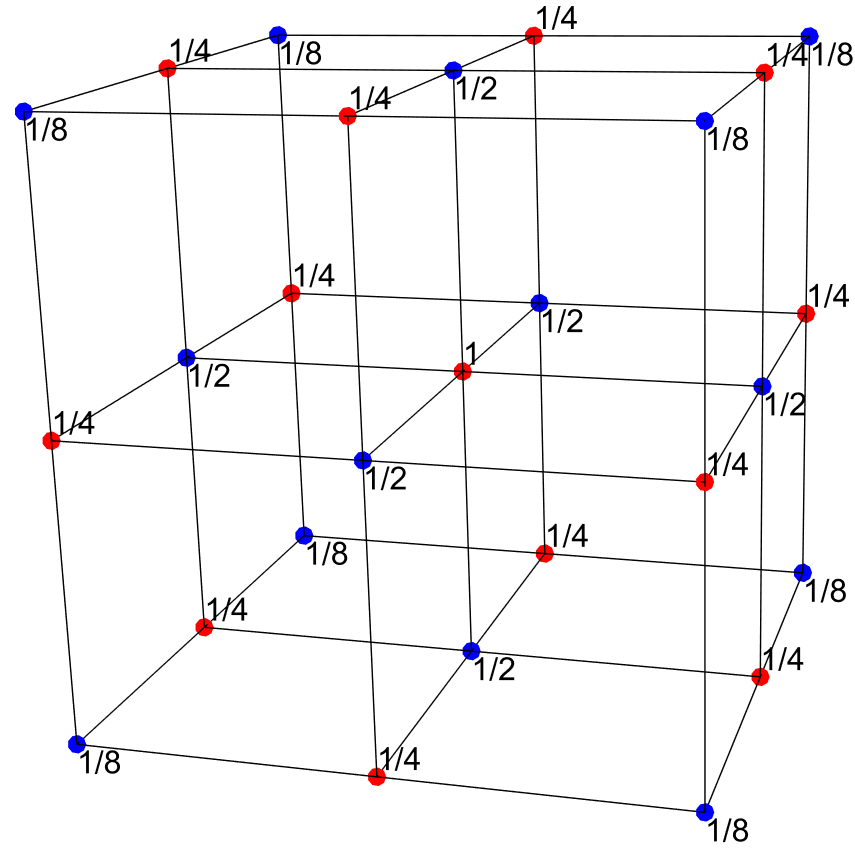
\includegraphics[width=0.4\textwidth,scale=0.4]{Cube}
    \caption[Elementarzelle eines Natriumchlorid-Kristalls.]{Elementarzelle eines Natriumchlorid-Kristalls.}\label{fig:nacl}
\end{figure}
Hierbei stellen die blauen Punkte negative und die roten Punkte positive Ladungen dar. Den Ladungen werden die Gewichte $1, \frac{1}{2}, \frac{1}{4}$ oder $\frac{1}{8}$
zugeteilt, je nachdem ob sie sich im Inneren, auf einer Seitenfläche, auf einer Kante oder auf einer Ecke des Würfels befinden. Dann verschwindet die Gesamtladung einer solchen
Elementarzelle. Nach H. M. Evjen \cite{key2} wird dann über die Potentiale der individuellen Zellen und nicht über die Potentiale der individuellen Ionen summiert, um die elektromagnetische Energie
eines einzelnen Gitterbausteins zu berechnen. Nach der sogenannten Evjen-Methode erfolgt dies über eine Summation über die Potentiale der einzelnen Ionen, wobei deren Ladung (wie oben bereits aufgeführt) gewichtet wird, je nachdem ob sie sich im Inneren,
auf einer Seitenfläche, auf einer Kante oder auf einer Ecke einer Elementarzelle befinden. Dieses Vorgehen ist äquivalent zu einer Summation über die Potentiale der Elementarzellen. Diese Methode
wird auch später im Code implementiert, wobei die Gewichtung der Ladungen durch eine entsprechende Benutzung von if-Statements erzielt wird.\newline Nun ist es unabdingbar, eine geeignete Summations-Formel zu finden.
Eine erste Vereinfachung des Problems besteht darin, den Gitterbaustein, auf den sich die zu berechnende elektromagnetische Energie bezieht, auf den Gitterplatz $(0,0,0)$ zu setzen. Für diesen
Gitterbaustein wird o.B.d.A ein Natrium-Ion (positiv geladen) (siehe Abbildung \ref{fig:nacl}) gewählt. Dieser Gitterbaustein stellt dann das Zentrum einer Elementarzelle dar. Damit vereinfachen sich die Einzelbeiträge der elektromagnetischen Energie zu
\begin{equation*}
    V_{i,j,k} = \frac{e}{4\pi\epsilon_0}\frac{e_{i,j,k}}{r_{i,j,k}}, \quad r_{i,j,k} = a \sqrt{i^2 + j^2 + k^2}
\end{equation*} wobei die Indizes $i,j,k$ den Gitterplatz eines anderen Ions beschreiben. Dann folgt sofort
\begin{equation*}
    V = \sum_{i,j,k=-n}^{n} V_{i,j,k} = \sum_{i,j,k=-n}^{n} \frac{e}{4\pi\epsilon_0} \frac{e_{i,j,k}}{a \sqrt{i^2 + j^2 + k^2}} = \frac{1}{4\pi\epsilon_0} \frac{e^2}{a} \sum_{i,j,k=-n}^{n} \frac{(-1)   ^{i+j+k}}{\sqrt{i^2 + j^2 + k^2}} = \frac{1}{4\pi\epsilon_0} \frac{e^2}{a} \alpha,
\end{equation*} wobei im vorletzten Schritt die alternierende Abfolge von positiven und negativen Ladungen im\newline Natriumchlorid-Kristall ausgenutzt wurde (negativer Beitrag,
wenn $i+j+k$ ungerade ist, was einer negativen Ladung (ungerade Anzahl an Gitterplatz-Schritten bis zum positiv geladenen Referenz-Ion) entspricht und positiver Beitrag, wenn $i+j+k$ gerade ist, was einer positiven Ladung (gerade Anzahl
an Gitterplatz-Schritten bis zum positiv geladenen Referenz-Ion) entspricht). $\alpha$ bezeichnet die sogenannte Madelung-Konstante für einen Natriumchlorid-Kristall. Der Term $i=j=k=0$ ist wegzulassen. Die Bezeichnung dieser Reihe mit einer Konstanten ist gerechtfertigt, da diese
Reihe für $n \to \infty$ konvergiert, wie D. Borwein, J. M. Borwein und K. F. Taylor 1985 zeigten \cite{key3}. Zunächst soll aber angemerkt sein, dass im Allgemeinen die Reihenfolge, in der die Terme summiert werden, eine Rolle bei der Konvergenz spielt. Jedoch zeigten
D. Borwein, J. M. Borwein und K. F. Taylor die Konvergenz der betrachteten Reihe $\alpha$ für expandierende Würfel, was dem physikalischen Sachverhalt eines Natriumchlorid-Kristalls entspricht.\newline Es stellt sich heraus, dass die Darstellung der obigen Reihe nicht allzu geeignet
für die Implementierung ist, da von $-n$ bis $n$ summiert wird. Eine Summation von $1$ bis $n$ ist wesentlich effizienter, weshalb im Folgenden eine entsprechende Formel angegeben wird (Beweis siehe \hyperref[sec:anhang]{Anhang}):
\begin{equation*}
    \sum_{i,j,k=-n}^{n}\frac{(-1)^{i+j+k}}{\sqrt{i^2 + j^2 + k^2}} = 8\sum_{i,j,k=1}^{n}\frac{(-1)^{i+j+k}}{\sqrt{i^2 + j^2 + k^2}} + 12\sum_{i,j=1}^{n}\frac{(-1)^{i+j}}{\sqrt{i^2 + j^2}} + 6\sum_{i=1}^{n} \frac{(-1)^{i}}{i}
\end{equation*}
Für eine endliche Zahl $n$ kann dieser Algorithmus nun mit den entsprechenden Gewichten (Evjen-Methode) implementiert werden. Das Ergebnis ist die Madelung-Konstante für einen Natriumchlorid-Kristall.\\ \\

\noindent 2. \textbf{KURZE ERKLÄRUNG ZUM CODE UND DANN DISKUSSION DER ERGEBNISSE}

\section*{Flacher Kristall}\label{sec:flach}

3. \textbf{NOCH ZU MACHEN}

\section*{Anhang}\label{sec:anhang}

Beweis für die Endformel der Madelung-Konstante aus dem \hyperref[sec:energie]{ersten Abschnitt}:
\begin{align*}
    \sum_{i,j,k=-n}^{n} \frac{(-1)   ^{i+j+k}}{\sqrt{i^2 + j^2 + k^2}} &= \sum_{i=-n}^{n} \sum_{j=-n}^{n} \sum_{k=-n}^{n} \frac{(-1)   ^{i+j+k}}{\sqrt{i^2 + j^2 + k^2}} \\
    &= \sum_{i=-n}^{n} \sum_{j=-n}^{n} \left(\sum_{k=-n}^{-1} \frac{(-1)^{i+j+k}}{i^2 + j^2 + k^2} + \frac{(-1)^{i+j}}{\sqrt{i^2 + j^2}} + \sum_{k=1}^{n} \frac{(-1)^{i+j+k}}{\sqrt{i^2 + j^2 + k^2}}\right) \\
    &= \sum_{i=-n}^{n} \sum_{j=-n}^{n} \left(2\sum_{k=1}^{n} \frac{(-1)^{i+j+k}}{i^2 + j^2 + k^2} + \frac{(-1)^{i+j}}{\sqrt{i^2 + j^2}}\right) \\
    &= \sum_{i=-n}^{n} \left(\sum_{j=-n}^{-1} \left(2\sum_{k=1}^{n} \frac{(-1)^{i+j+k}}{\sqrt{i^2 + j^2 + k^2}} + \frac{(-1)^{i+j}}{\sqrt{i^2 + j^2}}\right) + 2\sum_{k=1}^{n}\frac{(-1)^{i+k}}{\sqrt{i^2 + k^2}} + \frac{(-1)^{i}}{i}\right. \\
    &\left. \quad + \sum_{j=1}^{n}\left(2\sum_{k=1}^{n}\frac{(-1)^{i+j+k}}{\sqrt{i^2 + j^2 + k^2}} + \frac{(-1)^{i+j}}{\sqrt{i^2 + j^2}}\right)\right) \\
    &= \sum_{i=-n}^{n}\left(2\sum_{j=1}^{n}\left(2\sum_{k=1}^{n}\frac{(-1)^{i+j+k}}{\sqrt{i^2 + j^2 + k^2}} + \frac{(-1)^{i+j}}{\sqrt{i^2 + j^2}}\right) + 2\sum_{k=1}^{n}\frac{(-1)^{i+k}}{\sqrt{i^2 + k^2}} + \frac{(-1)^{i}}{i}\right) \\
    &= \sum_{i=-n}^{-1}\left(2\sum_{j=1}^{n}\left(2\sum_{k=1}^{n}\frac{(-1)^{i+j+k}}{\sqrt{i^2 + j^2 + k^2}} + \frac{(-1)^{i+j}}{\sqrt{i^2 + j^2}}\right) + 2\sum_{k=1}^{n}\frac{(-1)^{i+k}}{\sqrt{i^2 + k^2}} + \frac{(-1)^{i}}{i}\right) \\
    &\quad + 2\sum_{j=1}^{n}\left(2\sum_{k=1}^{n}\frac{(-1)^{j+k}}{\sqrt{j^2 + k^2}} + \frac{(-1)^{j}}{j}\right) + 2\sum_{k=1}^{n}\frac{(-1)^k}{k} \\
    &\quad + \sum_{i=1}^{n}\left(2\sum_{j=1}^{n}\left(2\sum_{k=1}^{n}\frac{(-1)^{i+j+k}}{\sqrt{i^2 + j^2 + k^2}} + \frac{(-1)^{i+j}}{\sqrt{i^2 + j^2}}\right) + 2\sum_{k=1}^{n}\frac{(-1)^{i+k}}{\sqrt{i^2 + k^2}} + \frac{(-1)^{i}}{i}\right) \\
    &= 2\sum_{i=1}^{n}\left(2\sum_{j=1}^{n}\left(2\sum_{k=1}^{n}\frac{(-1)^{i+j+k}}{\sqrt{i^2 + j^2 + k^2}} + \frac{(-1)^{i+j}}{\sqrt{i^2 + j^2}}\right) + 2\sum_{k=1}^{n}\frac{(-1)^{i+k}}{\sqrt{i^2 + k^2}} + \frac{(-1)^{i}}{i}\right) \\
    &\quad + 2\sum_{j=1}^{n}\left(2\sum_{k=1}^{n}\frac{(-1)^{j+k}}{\sqrt{j^2 + k^2}} + \frac{(-1)^{j}}{j}\right) + 2\sum_{k=1}^{n}\frac{(-1)^{k}}{k}
\end{align*} Umbenennung von Laufvariablen und Umsortierung der Terme liefert schließlich:
\begin{equation*}
    \sum_{i,j,k=-n}^{n}\frac{(-1)^{i+j+k}}{\sqrt{i^2 + j^2 + k^2}} = 8\sum_{i,j,k=1}^{n}\frac{(-1)^{i+j+k}}{\sqrt{i^2 + j^2 + k^2}} + 12\sum_{i,j=1}^{n}\frac{(-1)^{i+j}}{\sqrt{i^2 + j^2}} + 6\sum_{i=1}^{n} \frac{(-1)^{i}}{i}
\end{equation*} Es wurde dabei benutzt, dass der Term $i=j=k=0$ wegzulassen ist.\newpage

\listoffigures

\bibliographystyle{unsrt}
\bibliography{refs}

\end{document}